%!TEX root = ../thesis.tex
\chapter{Background}
\label{ch:background}

\section{Hexapods} \label{sec: Hexapods}
Hexapods are a class of robots featuring 6 legs, inspired by the locomotion of insects and arachnids.
Through millions of years of evolution these organisms developed efficient locomotion strategies \parencite{neville2006bipedal}, making them a rich source of inspiration for robotics.
By emulating the biomechanics and behaviour of insects, researchers and engineers aim to create versatile and robust robotic systems capable of navigating challenging terrain \parencite{irawan2011optimal, ouyang2021adaptive, schilling2013walknet}.

Most commonly, each leg of a hexapod consists of 3 segments named coxa, femur and tibia, equivalent to their biological counterparts.
The individual segments are connected by 3 1-DoF (degrees of freedom) joints, each actuated by an electric servo motor.
The first joint, hereafter named \textalpha-joint, connects the coxa to the thorax(body) and moves in parallel to the ground, thus being responsible for the longitudinal placement of each leg.
Coxa and femur are connected by the \textbeta-joint, while the femur and tibia are connected by the \textgamma-joint. 
These joints move orthogonal to the movement plane of the \textalpha-joint. Together, they are responsible for the lateral positioning of each leg.
The nomenclature we use use in this thesis to label the joints and leg segments was adopted from the works of \cite{schilling2013walknet} and \cite{HeterarchicalArchitectureSchilling}.
\begin{figure}[h]
	\centerline{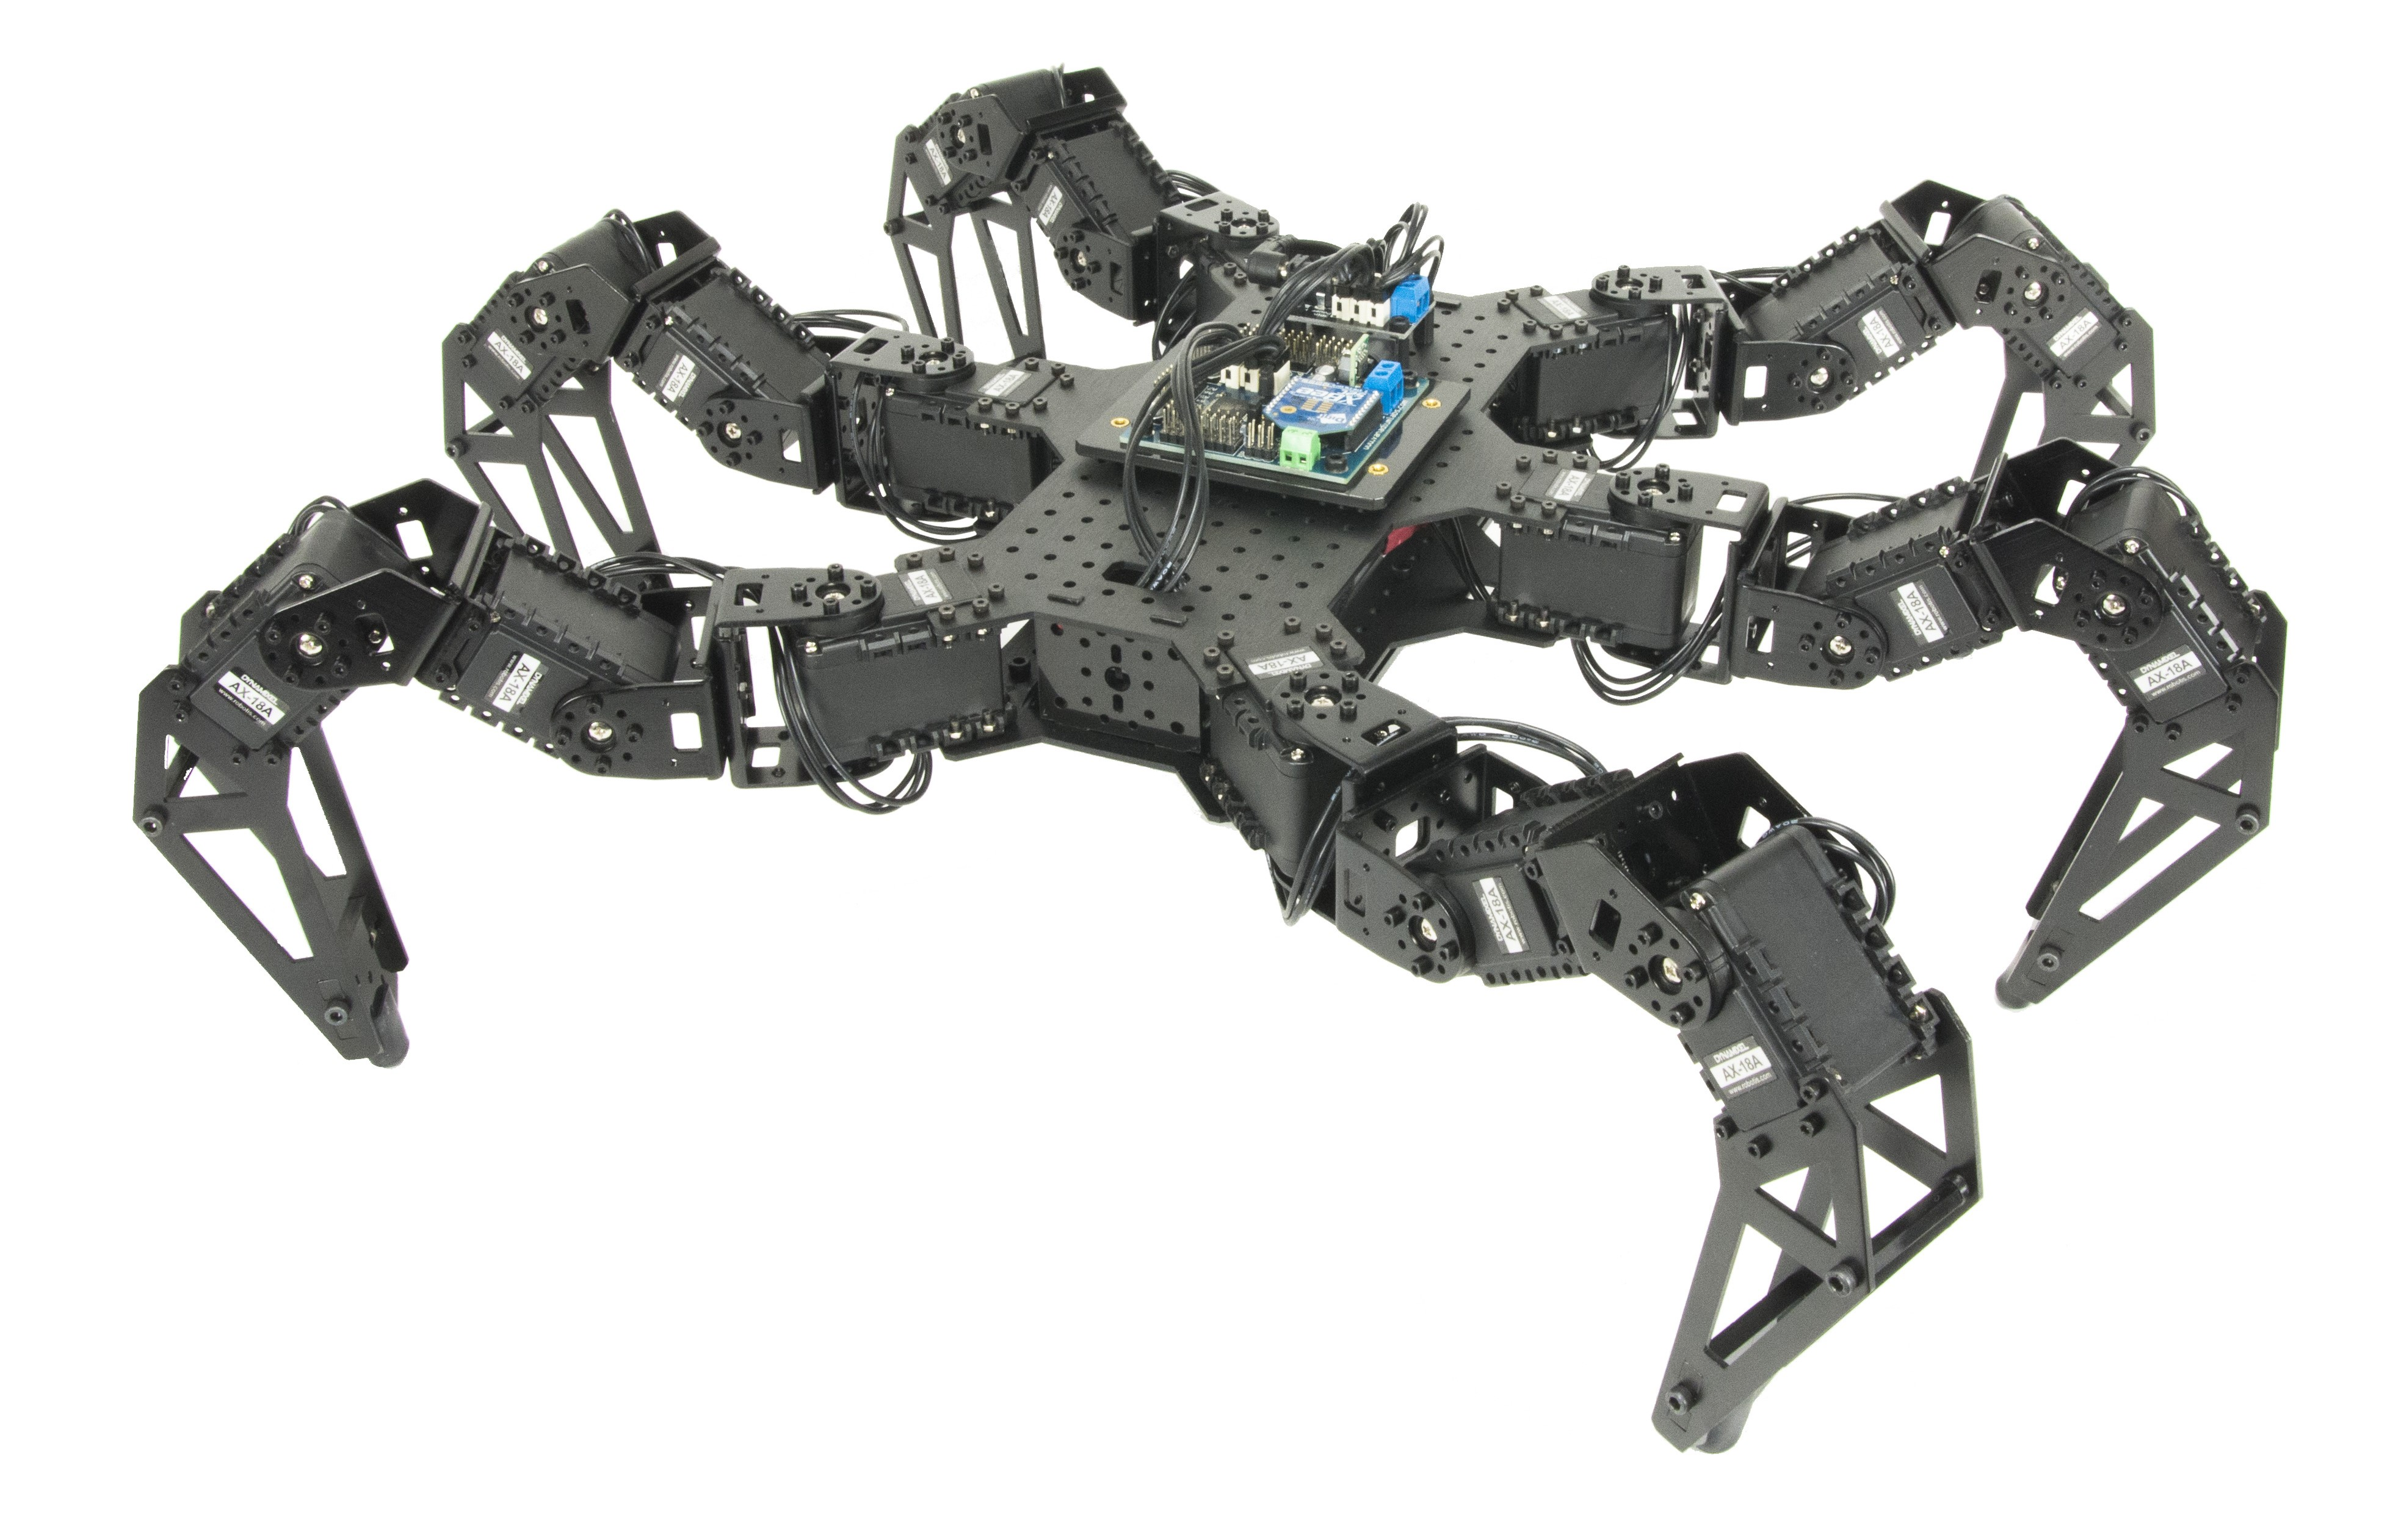
\includegraphics[scale=0.04]{phantomX_III_overview}}
	\caption{PhantomX MKIII hexapod, predecessor of MKIV used here [\cite{PhantomX_MKIII}]}
	\label{figure: PhantomX MKIII}
\end{figure}

\todo{"Gait Self-learning for Damaged Robots Combining Bionic Inspiration and Deep Reinforcement Learning" for parameters of hexapod}

\todo{Maybe add image of stick insect}

\todo{CITATIONS}

\section{MATLAB}
\textit{MATLAB\textsuperscript{\textregistered}} is a numerical computing environment and programming language, developed by the company \textit{MathWorks\textsuperscript{\textregistered}}.
It is widely used by researchers and engineers alike in applications such as data analysis and visualisation, algorithm development or the creation of virtual models.
The MATLAB environment provides a multitude of apps and toolboxes to support different domains, for example model-based design, machine learning, signal processing or hardware co-simulation \parencite{MATLAB}.

\hiddensubsection{Simulink}
\textit{Simulink\textsuperscript{\textregistered}} is a \textit{MATLAB\textsuperscript{\textregistered}}-based graphical block-diagramming tool developed by the company . 
It is a widely used tool which plays a crucial role in various engineering and research disciplines.
It provides the user with a versatile platform to design, simulate and analyse complex dynamic systems.

Simulink offers an expansive library of predefined blocks that represent different components and behaviours.
The user connects these blocks using edges called signal lines to transport data between them.
Blocks transform the data provided by the inputs and output the transformed data to other blocks connected downstream.
Their behaviour can be discrete, like a switch or logic gate which activate when specific signals are pulled high, or represent more complex and continuous functions such as integrators, derivatives or sine waves.

An arrangement of blocks can be encapsulated into a subsystem, thus creating different levels of abstraction.
To enable simple reuse of components, subsystems can be placed in custom libraries.
If such a library object is modified, each linked copy of this subsystem receives the update as well, preventing the developer from having to edit each copy individually.
At any step in the development process, a model can be simulated and analysed.
To be able to better analyse a model,the value of any signal lines can be plotted over time and the simulation speed can be slowed down.
An example of a simple Simulink model can be seen in \ref{figure: Simulink bouncing ball example}.
The model simulates the behaviour of an elastic ball which, under the influence of (earth's) gravity, accelerates downwards and repeatedly bounces of an imaginary plane.
The ball looses energy over time, as represented by the coefficient of restitution.
To visualize the systems dynamics, the balls velocity and speed are logged and plotted, as can be seen by the small symbols next to the respective signal lines.

\begin{figure}[h!]
	\begin{subfigure}{.5\textwidth} % this sets the figure to be max half the width of the page
		\centering
		% include first image
		\includesvg[scale=0.5]{Simulink/BouncingBallExample_Simulink.svg}  % this sets the image to fill 90% of the available space -> 45% of the line width in total. 
		\caption{}
		\label{figure: Simulink bouncing ball model}
	\end{subfigure}
	\begin{subfigure}{.5\textwidth}
		\centering
		% include second image
		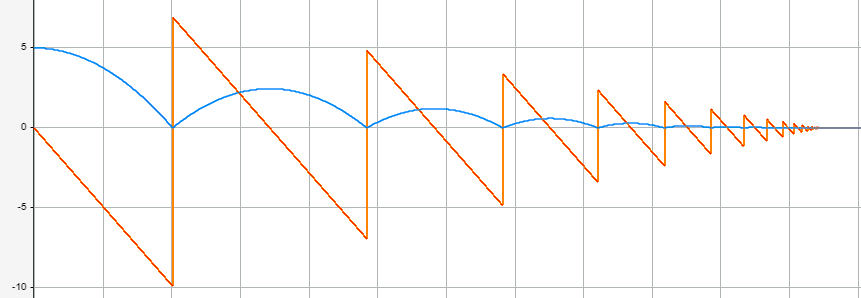
\includegraphics[width=\linewidth]{Simulink/BouncingBall_PositionAndVelocity.png}  
		\caption{}
		\label{figure: Simulink bouncing ball graphs}
	\end{subfigure}
	\caption[Simulink bouncing ball example]{(a) Simulink model of a bouncing ball created suing standard library blocks. (b) Graphs depicting the balls velocity(orange) and position(blue).}
	\label{figure: Simulink bouncing ball example}
\end{figure}


\hiddensubsection{Simscape}
\textit{Simscape\textsuperscript{\texttrademark}} is a Simulink block library developed by \textit{MathWorks\textsuperscript{\textregistered}} enabling the construction of physical systems within the Simulink environment.
Utilizing Simscape, it is possible to model and simulate systems such as electric circuits, hydraulics or classical mechanics all within a unified simulation environment.
The library offers a large variety of predefined components like resistors, capacitors, springs, dampers, etc.
To understand the model we develop in this thesis, Simscape's mechanical components are of the most interest, especially coordinate frames, rigid transforms, joints and rigid bodies.

\begin{figure}[h!]
	\centering
	\centerline{\includesvg[scale=0.8]{Simulink/BouncingBallExample_Simscape.svg}}
	\caption[Simscape bouncing ball example]{Simulink model of the same bouncing ball system as in \ref{figure: Simulink bouncing ball model}, but created using solely Simscape blocks. The simulation of this system is provided in \cite{VIDEO 1}. }
	\label{figure: Simscape Bouncing Ball Example}
\end{figure}

Coordinate frames are at the base of every Simscape model.
They can be attached to each other using rigid transforms or joints.
Edges similar to the basic Simulink signal lines are used to connect the individual blocks.
These lines do not transport plot-able signal however, but rather represent the structure of the Simscape model.
Joints allow for different degrees of freedom between two frames, depending on what constraints should be imposed on the system.
Two frames connected by a joint are called base and follower frame.
When a joint is actuated, either by an external or internal force, the follower frame moves relative to the base frame \parencite{thilderkvist2015motion}.
As already mentioned in the previous sentence, joints can be actively actuated by providing them with a scalar torque signal.
It is also possible to modify various joint parameters such as internal joint friction, joint limits and spring stiffness, which we will explain in chapter \ref{ch:methods}.

Rigid transforms translate and/or rotate coordinate frames without allowing for any degree of freedom.
They are used to define the initial position and orientation of a frame.
Rigid bodies can be attached to the already existing coordinate frames, providing shape, mass and inertia to the system.
If multiple of these are present in a simulation, the shape of a rigid body can also act as collision geometry, allowing different bodies to collide and interact with each other.
If a component is required which is not yet represented by a block in the library, Simscape offers a MATLAB based language to enable text-based development of custom components.
The description of the Simscape library in this section roughly follows the official documentation \parencite{matlabSimscapeDocumentation}.

As an example, the same bouncing ball system as shown in \ref{figure: Simulink bouncing ball model} can be seen in \ref{figure: Simscape Bouncing Ball Example} constructed using only blocks from the Simscape library. When simulating this model, a 3D animation of the bouncing ball is generated which can be slowed down, replayed or saved for later analysis.
\todo{CITATIONS ?}


\section{Insect Locomotion}
The locomotion of insects, more specifically arthropods,\todo{CITATION} serves as a remarkable source of inspiration for the field of hexapod robotics.
There exists a vast amount of papers studying the movement patterns of these insects.
Common research subjects include LATIN(stick insect), LATIN(fruit fly) or LATIN(cockroaches).\todo{CITATIONS}
The probably most essential aspect of the locomotion of an arthropod is the "Swing-Stance Cycle", as depicted in \ref{figure: Stick insect leg}.


\begin{figure}[h]
	\centerline{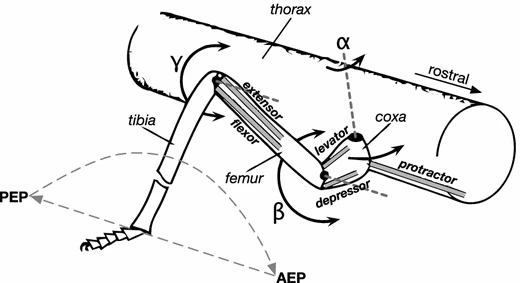
\includegraphics[scale=0.4]{morphologyOfStickInsect_sketch}}
	\caption{Morphologic drawing of a stick insect leg (\cite{schilling2013walknet} [Fig.1]).}
	\begin{footnotesize}
		Angle $\alpha$ represents the position of the thorax-coxa joint, angle $\beta$ describes the position of the coxa-femur joint and angle $\gamma$ represents the position of the femur-tibia joint.
		These joints are actuated with three pairs of muscles, protractor-retractor, levator-depressor and extensor-flexor respectively.
		Also depicted are the posterior extreme position(PEP), defined as the rearmost point of the movement cycle, and the anterior extreme position(AEP), the foremost point in the cycle.
		Dashed lines depict the swing and stance movement between PEP and AEP.
	\end{footnotesize}
	
	\label{figure: Stick insect leg}
\end{figure}

As its name suggests, the movement cycle of an arthropod leg is divided into two distinct phases, the swing phase and the stance phase.
While in stance, the leg is constantly in contact with the ground and bears a partial load of the insects weight.
During this phase the leg moves backwards relative to the body, from the AEP (Anterior Extreme Position) to PEP (Posterior Extreme Position) and pushes the insect forward.
The AEP describes the foremost point a leg reaches during the movement cycle, the PEP the rearmost point.
When the leg reaches the PEP, the swing phase begins and it is lifted of the ground and moved forward.
While the stance phase is responsible for holding the insect up and moving it forward until reaching the PEP, the swing phase is needed to reposition the leg towards the AEP to start the cycle again.
The complete cycle can be described as a pushing phase (Stance) and a repositioning phase (Swing).

\todo{CITATIONS}


\section{Inverse Kinematics}
Inverse Kinematics (IK) is a mathematical approach predominately used in the fields of robotics and computer graphics.
It describes the process of calculating the joint angles required to place the end of a kinematic chain, the so called the end-effector, at a given position and orientation in space.
A kinematic chain is an abstract description of a chain consisting of joints and links, such as a robotic manipulator or the arm of a human 3D model.
Solving inverse kinematics can be a challenging task, especially for robots with many DoF and complex joint constraints.
The difficulty arises from the fact that there can exist multiple solutions (multiple sets of joint angles) to achieve the same end-effector pose.
Some of which some may be physically feasible while others might lead to collisions or instabilities.\\
There exist two primary techniques for solving the inverse kinematics problem, analytical and numerical methods \parencite{inverseKinematicsIllinois}:
\todo{Citations}
\todo{Mention forward kinematics ?}

\subsection{Analytical IK}
Analytical solution methods are based on trigonometric equations derived from the geometric and kinematic parameters of the manipulator arm, such as the link length, joint type and joint constraints.
An example of such derivations is presented at a later point in this work, see \ref{subsubsec: IK Solver}.
They provide exact solutions to the problem and only use minimal computational resources.
Although very efficient and precise, the analytical approach is generally only feasible for kinematic chains with a small number of DoF.
If the kinematic chain contains redundant DoFs, meaning it possesses more DoF than the dimension of the workspace it is in, there can exist multiple or even infinite solutions to the IK problem \parencite{inverseKinematicsIllinois}.
Such systems potentially lack closed-form expressions for solutions, making it infeasible to apply analytical solution methods.

\subsection{Numerical IK}
Numerical solution methods use iterate approaches to approximate the joint angles and converge towards a solution over several iterations of their algorithm.
At the start of the process, numerical methods begins with an initial guess.
This guess can be based on the manipulators geometry, joint limits, previously obtained solutions and other heuristics.
Using the estimated joint angles, the would-be position of the end-effector is calculated (forward kinematics) and the error between the desired pose and the currently obtained pose is determined.
Based on this, the joint angle estimates are adjusted, aiming to reduce the error and bring the end-effector closer to the desired pose.
This process is repeated until the error meets the predefined tolerances.
The joint angles calculated during the final iteration are then considered a solution to the problem.
Although the basic principle of iterative error-minimization is always present in numerical solution methods, the exact process of minimization is much more complex than described here and there exist numerous different techniques on how to achieve this goal, such as Cyclic Coordinate Descent, Jacobian Inverse or FABRIK. \todo{CITATION}
Numerical methods can be applied to a wide variety of inverse kinematic problems and are not limited by the number of DoF like analytical methods.
Due to their iterative nature they are generally significantly more computationally expensive, given the same problem, than their analytical counterparts \parencite{aristidou2018inverse, inverseKinematicsIllinois}.

Both inverse kinematics methods are used extensively in industry and research, depending on the specific project and its requirements.


\section{PID Controller}
The \textbf{P}roportional-\textbf{I}ntegral-\textbf{D}erivative (PID) controller is the most commonly used feedback control system in many modern industries \parencite{aastrom2002control}.
A feedback control system aims to regulate a control variable towards a desired setpoint by adjusting its output according to the currently measured process variable.
In most cases this process variable corresponds to a real world variable such as the speed of a motor, the liquid-level inside a tank or the temperature of a furnace.
The architecture of a PID controller consists of three terms, a proportional, integral and derivative term, which together compute the controlled output based on the error between setpoint and current process variable.
Focusing on digital PID controllers, the process of error calculation and control variable adjustment is done at a discrete, fixed rate, also referred to as a time step.
There also exist implementations of this control loop type using analogue electronics which generate a continuous control signal, but these are of no concern for the content of this thesis.
In the following section we will describe the operation of a (digital) PID controller in detail:

\begin{figure}[h]
	\centerline{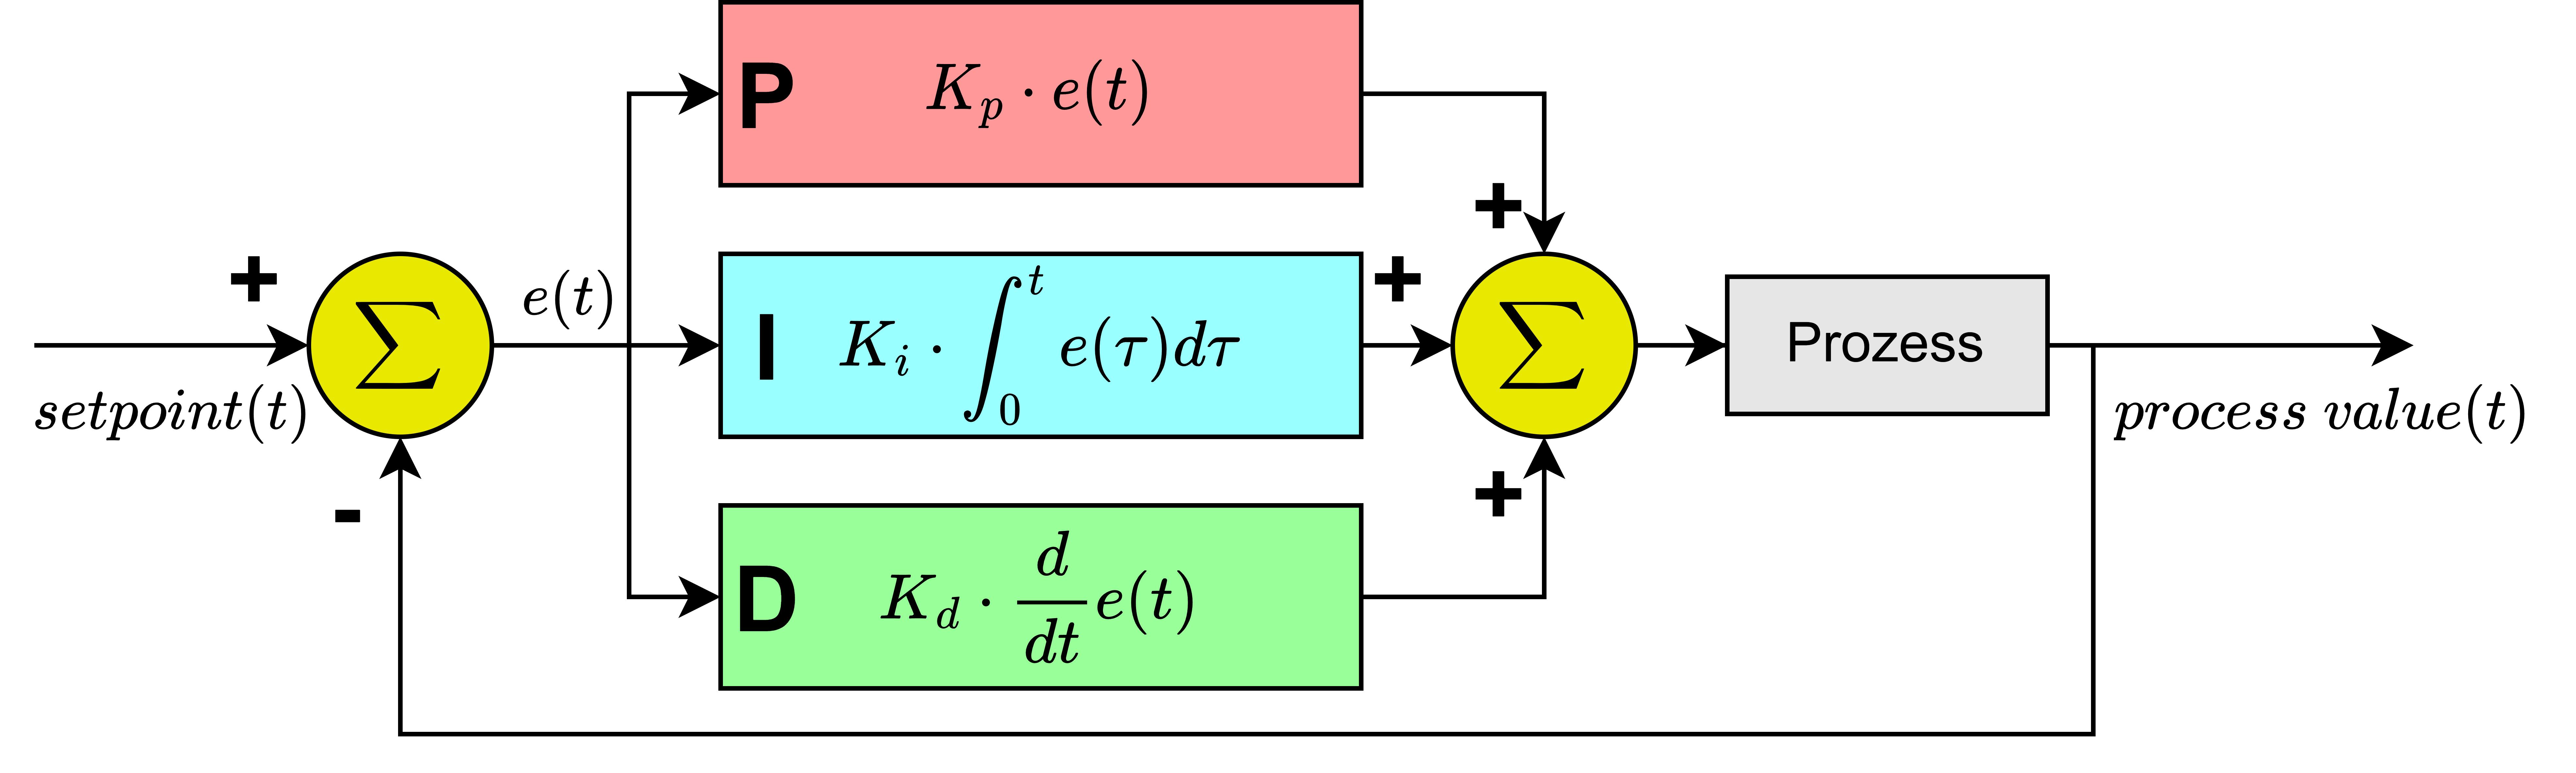
\includegraphics[scale=0.05]{PID_Controller}}
	\caption{Illustration of a basic PID Controller}
	\label{figure: PID Controller}
\end{figure}

\todo{Change d and dt to /partial in pid graphic}

At each time step the controller first calculates the error between its setpoint and the currently measured process variable: 
\[
	Error(t) = setpoint - process\ variable(t)
.\]
Following this, the controller then determines the proportional, integral and derivative term based on this error.

The proportional term $P(t)$ is calculated by multiplying the error by a constant factor, the so called proportional gain $K_p$.
This term contributes to the control output, as its name suggests, proportional to the magnitude of the error.
$P(t)$ is given by:
\[
	P(t) = K_p \cdot Error(t)
.\]
The integral term $I(t)$ takes into account the sum of past errors to address any long term bias/ constant error present inside of the controlled system.
Such a bias might for example be the gravitational pull a drone experiences while it is supposed to stay at a constant height.
The term is able to eliminate long-term errors that can not be accounted for by $P(t)$.
It is calculated by integrating the error over time and multiplying it with the integral gain $K_i$.
$I(t)$ is given by:
\[
	I(t) = K_i \cdot \int_{0}^{t} Error(\tau) \,d\tau
.\]
The derivative term $D(t)$ anticipates the errors future behavior by determining the errors rate of change.
It prevents the controller from overshooting and oscillating by dampening the control response.
$D(t)$ is calculated by multiplying the errors rate of change with the constant derivative gain $K_d$.
It is given by:
\[
	D(t) = K_d \cdot \frac{\partial}{\partial t}(Error(t))
.\]
The final output of the controller at time $t$ is then given by the sum of all three terms:
\[
	Control\ Output(t) = P(t) + I(t) + D(t)
.\]
The calculated control output is fed into the controlled system or process and the PID controller calculates the next control value.

As an additional note, in real-world applications the derivative term is almost never implemented as a pure derivative, as it would be extremely sensitive to noise.
Instead, a so called filter coefficient ($N$) is utilised to counteract this sensitivity.
The modified term acts as a first-order, low pass filter, attenuating high frequency noise.
This term acts equivalently to a derivative up to a given cutoff frequency[Hz] given by: $\frac{N}{2\pi}$ \todo{Filter coeff. and cutoff frequency}.

The performance of a PID controller greatly depends on the values of its parameters $K_p$, $K_i$ and $K_d$ (and N).
To achieve desired traits like a fast response time and minimal overshooting or oscillation, these parameters have to be carefully tuned. 
This tuning process can be done manually via trial-and-error or methodically using a tuning algorithm.

Summarizing, a PID controller continuously repeats the process of error calculation and adjustment, thus forming a closed-loop system which aims to minimize the error and thus approach the setpoint as close as possible.

\todo{CITATIONS}


\section{Reinforcement Learning} \label{sec: Reinforcement Learning}

Reinforcement Learning (RL), besides Supervised and Unsupervised Learning, is one of the three major branches in the field of Machine Learning.
The basic underlying principle of RL is to learn how a scalar reward signal can be cumulatively maximized without being told which path might lead to the highest reward \parencite{sutton2018reinforcement}.
On an abstract level, learning takes place by letting an agent (or multiple agents) take sequences of actions in an environment, then improving the actions to be taken next time, based on the obtained experiences.
This process is called "training" and it is essential to the operation of RL.
Some of the principles used in RL are inspired by behavioral psychology, where learning is mainly driven by the consequences of the actions taken \parencite{sutton2018reinforcement, joshi2021reinforcement}.
To gain a deeper understanding of Reinforcement Learning, we will examine the three most important elements of the training process in detail:

\begin{figure}[h]
	\centerline{
\includegraphics[scale=0.075]{RL_Overview}}
	\caption{Sketch illustrating the basic concept of Reinforcement Learning}
	\label{figure: RL Illustration}
\end{figure}

The agent, as seen in \ref{figure: RL Illustration}, is the entity which learns, it takes actions $A_t$ in the environment and receives observations $O_t$ and the reward signal $R_t$ from the environment.
An agent always acts according to its current policy.
A policy is roughly defined as a mapping of all perceived environmental states to the actions to be taken by the agent when in a given state.
It fully  describes the way a learning agent behaves at any given point(in time) in the learning process.\parencite{sutton2018reinforcement} \parencite{silver2015}
The agents policy is continually updated during the training process, always trying to improve the actions taken by the policy towards a higher expected reward.
%MATLABs \textit{Reinforcement Learning Toolbox} provides several different RL agents, some of which will will go into more detail about later.

The environment is defined as the space in which the agent tries to improve its policy by taking actions and learning from them.
It defines the problem which the RL agent is supposed to solve by learning a policy.
The problem definition can range from robotic control tasks such as bipedal walking or autonomous driving over playing video games all the way to advertisement or news recommendations.
Every problem for which it is possible to define a reward function that accurately determines the agents performance, RL can be applied to \parencite{silver2015}.
The sole way the agent is able to influence the environment is by taking actions in it.
The environment receives the actions chosen by the agent and computes the resulting environmental state and the amount of reward the agent receives for the state it is in.
It provides the reward and observations about the environment to the agent.

\begin{comment}
%Discrete vs. Continuous action space in RL learning: 
Using the RL toolbox, 2 distinct types of environment are provided which differ in the definition of their action space.
If an environment has a discrete action space, it means that there exists countable, discrete actions which can be taken.
Discrete action spaces are used when the number of possible actions is limited and known in advance.
An example of such an environment would be a game of chess; for each turn there is a finite number of available moves.
Continuous action spaces on the other hand have a continuum of actions which can be taken and are used when the number of possible actions is infinite, such as the movement possibilities of a robotic arm.	
\end{comment}

The reward function/ reward signal is a scalar function which determines the agents performance given a predefined goal.
At each time step, the function is evaluated and the scalar output, the reward, is sent to the agent.
The maximization of this reward is the sole objective of the agent \parencite{silver2015}.
Due to the reward being the only metric which defines which agent behaviour is good and bad, it is important to define this function well.
If the reward function is poorly defined, the agent will perform poorly as well.
The reward function is considered part of the environment.
\parencite{sutton2018reinforcement}
\todo{expand to include MDP, RL agorithms, etc. ?}

\begin{comment}

\parencite{weng2018bandit}
\parencite{sutton2018reinforcement}

Model-Free vs. Model ?


\begin{definition*}
	A policy $\pi$ is a distribution over actions given states,\\
	$\pi(a|s) = \mathbb{P}(A\textsubscript{t} = a\,|\,S\textsubscript{t} = s)$
\end{definition*}
A policy fully defines an agents behavior. 
\todo{Cite David Sijlver Lec. 2}

A value function, in contrast to a reward function which immediately rewards good actions, defines what is good long term. 
Rewards only define the immediate desirability of environmental states, a value function takes into account states which are likely to follow a given state and the rewards available in those states.
A state might immediately yield a low reward, but if it is likely followed by states which yield high rewards, it can still possess a high value.
This can also be true for the opposite, a state has a high immediate reward, but is likely only followed by states which yield low rewards. Thus the state has a low value \parencite{sutton2018reinforcement}.

Some methods of solving RL problems also consider a model of the environment. This means that the approach has a way of planning ahead, such as predicting the next environmental state and reward.
Methods which use a model are called model-based, methods which explicitly only learn by trial and error model-free\parencite{sutton2018reinforcement}.

Offline vs. Online Reinforcement Learning: 
RL agents labeled as offline only learn from a fixed dataset which has been acquired before starting the training process.
The agent itself does not interact with the environment, only learning on historical data.
Online RL agents on the other side learn while actively interacting with the environment.
They decide, act and receive feedback all in real-time and learn from the consequences of their actions \parencite{schrittwieser2021online}.


Markov Property: "The future is independent of the past given the present"
The current state contains all relevant information to make predictions about the future
\begin{definition*}
	State S\textsubscript{t} is \textbf{\textit{Markov}}, if and only if
	$ P(S\textsubscript{t+1} | S\textsubscript{t}) = P(S\textsubscript{t+1} | S\textsubscript{1},...,S\textsubscript{t}) $.
\end{definition*}

Markov Process:
A Markov Process is a memory-less random process, i.e. a sequence of random states S\textsubscript{1}, S\textsubscript{2},... that have the Markov property.

\begin{definition*}
	A Markov Process (or Markov Chain) is a tuple $\langle\mathcal{S,P}\rangle$ where
		\begin{itemize}
		\item $\mathcal{S}$ is a (finite) set of states that have the Markov property
		\item $\mathcal{P}$ is a state-transition probability matrix,\\
		$\mathcal{P}\textsubscript{ss'} = \mathbb{P}[S\textsubscript{t+1} = s'|S\textsubscript{t}=s] $
	\end{itemize}
\end{definition*}
\todo{Cite David Silver RL course Lec. 1-2 for everything about Markov}

Markov Decision Process(MDP):

$\rightarrow$ Hexapod locomotion can be considered a MDP, see: \parencite{ouyang2021adaptive} [p.7, 4.1]
$\rightarrow$ Try DDPG for RL, allegedly widely used in robotics \parencite{ouyang2021adaptive}


Agents applicable for continuous action spaces: 
\begin{itemize}		
	\item DDPG: Deep Deterministic Policy Gradient
	Model-free, continuous action space, actor-critic (Look at \parencite{trotta2022walking})
	\item TD3: Twin-Delayed Deep Deterministic Policy Gradient (more complex improvement to DDPG)
	Model-free, continuous action space, actor-critic
	\item PPO: Proximal Policy Optimization (more stable updates, but longer training)
	Model-free, continuous or discrete action space; policy gradient rl-method
	\item SAC: Soft Actor-Critic (more complex improvement of DDPG generating stochastic policies)
	Model-free, continuous action space, actor-critic
	\item TRPO: Trust Region Policy Optimization(more complex version of PPO, more robust for deterministic environments with fewer iterations)
\end{itemize}
\end{comment}